\graphicspath{{images_low_res/}}

\section{Background of Research}
\label{sec:background}

\subsection{A Comparison of Methods for Screening Strain Fitness }


% \begin{figure}
%    \centering
%    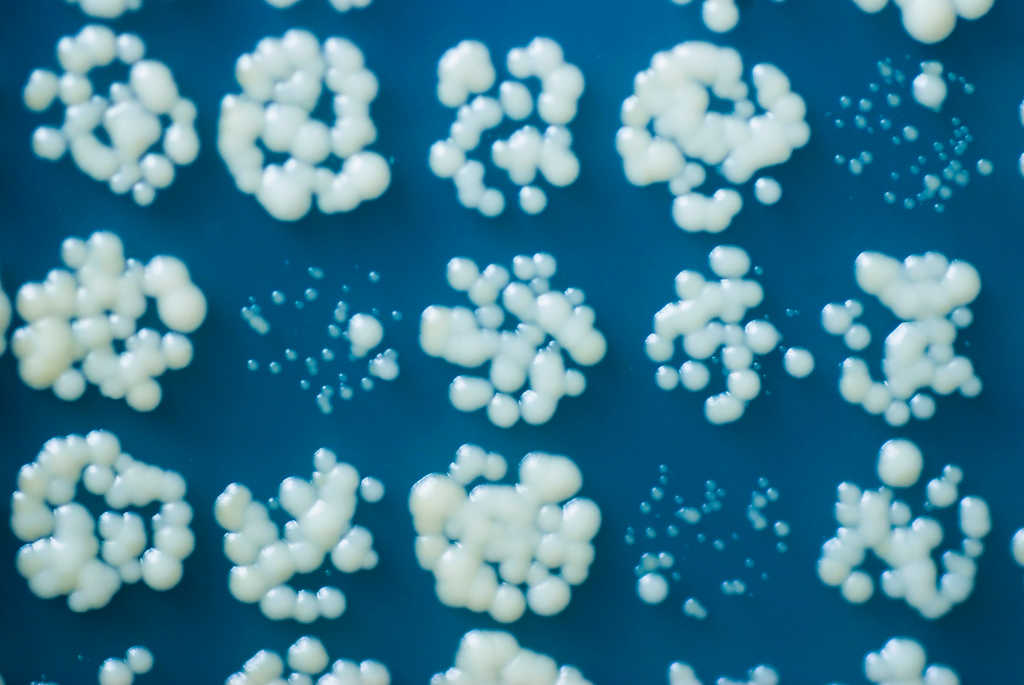
\includegraphics[width=\linewidth]{5658435523_c2e43729f1_b}
%    \captionof{figure}{An example QFA agar.}
% \end{figure}

\begin{Figure}
  \centering
  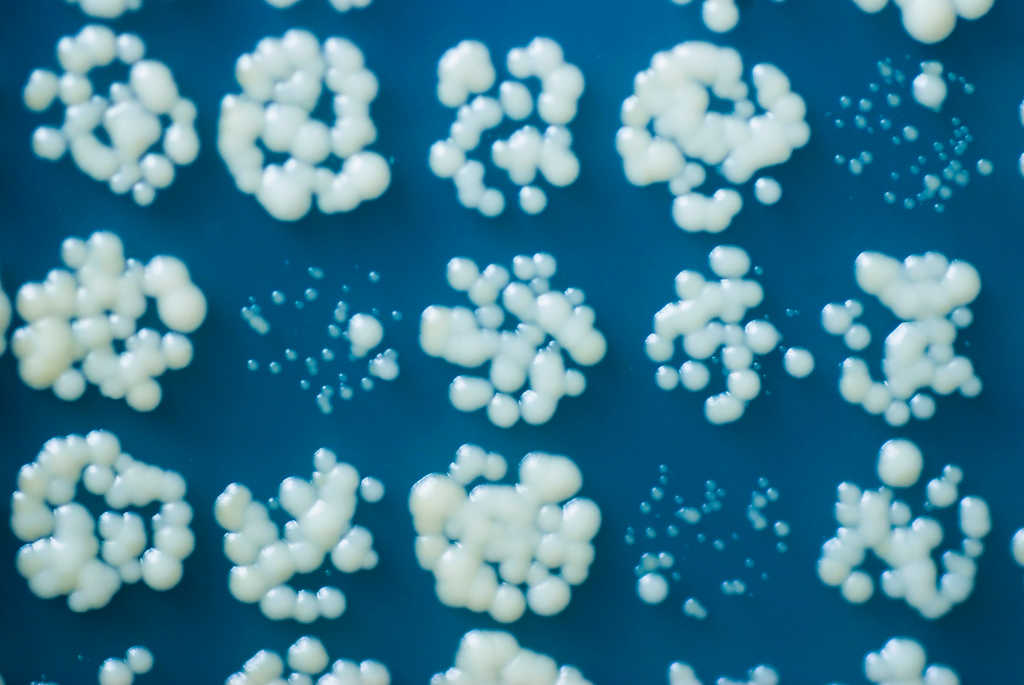
\includegraphics[width=\linewidth]{5658435523_c2e43729f1_b}
  \captionof{figure}{An image of 15 cultures on a section of solid agar
    from a QFA procedure. Image taken ??with permission?? from the Colonyzer GitHub repo
    https://github.com/CnrLwlss/Colonyzer \citep{Lawless2010}}
\end{Figure}

Some lines of test about the figuresSome lines of test about the figuresSome lines of test about the figuresSome lines of test about the figuresSome lines of test about the figuresSome lines of test about the figuresSome lines of test about the figuresSome lines of test about the figuresSome lines of test about the figuresSome lines of test about the figuresSome lines of test about the figuresSome lines of test about the figuresSome lines of test about the figuresSome lines of test about the figuresSome lines of test about the figuresSome lines of test about the figuresSome lines of test about the figuresSome lines of test about the figuresSome lines of test about the figuresSome lines of test about the figuresSome lines of test about the figuresSome lines of test about the figuresSome lines of test about the figuresSome lines of test about the figuresSome lines of test about the figuresSome lines of test about the figuresSome lines of test about the figuresSome lines of test about the figuresSome lines of test about the figuresSome lines of test about the figuresSome lines of test about the figuresSome lines of test about the figuresSome lines of test about the figuresSome lines of test about the figuresSome lines of test about the figuresSome lines of test about the figuresSome lines of test about the figuresSome lines of test about the figuresSome lines of test about the figuresSome lines of test about the figuresSome lines of test about the figuresSome lines of test about the figuresSome lines of test about the figuresSome lines of test about the figuresSome lines of test about the figuresSome lines of test about the figuresSome lines of test about the figuresSome lines of test about the figuresSome lines of test about the figuresSome lines of test about the figuresSome lines of test about the figuresSome lines of test about the figuresSome lines of test about the figuresSome lines of test about the figuresSome lines of test about the figuresSome lines of test about the figuresSome lines of test about the figuresSome lines of test about the figuresSome lines of test about the figuresSome lines of test about the figuresSome lines of test about the figuresSome lines of test about the figuresSome lines of test about the figuresSome lines of test about the figures.
Some lines of test about the figuresSome lines of test about the figuresSome lines of test about the figuresSome lines of test about the figuresSome lines of test about the figuresSome lines of test about the figuresSome lines of test about the figuresSome lines of test about the figuresSome lines of test about the figuresSome lines of test about the figuresSome lines of test about the figuresSome lines of test about the figuresSome lines of test about the figuresSome lines of test about the figuresSome lines of test about the figuresSome lines of test about the figuresSome lines of test about the figuresSome lines of test about the figuresSome lines of test about the figuresSome lines of test about the figuresSome lines of test about the figuresSome lines of test about the figuresSome lines of test about the figuresSome lines of test about the figuresSome lines of test about the figuresSome lines of test about the figuresSome lines of test about the figuresSome lines of test about the figuresSome lines of test about the figuresSome lines of test about the figuresSome lines of test about the figuresSome lines of test about the figuresSome lines of test about the figuresSome lines of test about the figuresSome lines of test about the figuresSome lines of test about the figuresSome lines of test about the figuresSome lines of test about the figuresSome lines of test about the figuresSome lines of test about the figuresSome lines of test about the figuresSome lines of test about the figuresSome lines of test about the figuresSome lines of test about the figuresSome lines of test about the figuresSome lines of test about the figuresSome lines of test about the figuresSome lines of test about the figuresSome lines of test about the figuresSome lines of test about the figuresSome lines of test about the figuresSome lines of test about the figuresSome lines of test about the figuresSome lines of test about the figuresSome lines of test about the figuresSome lines of test about the figuresSome lines of test about the figuresSome lines of test about the figuresSome lines of test about the figuresSome lines of test about the figuresSome lines of test about the figuresSome lines of test about the figuresSome lines of test about the figuresSome lines of test about the figures.

\end{multicols}
\graphicspath{{images_low_res/}}
\begin{Figure}
  \centering
  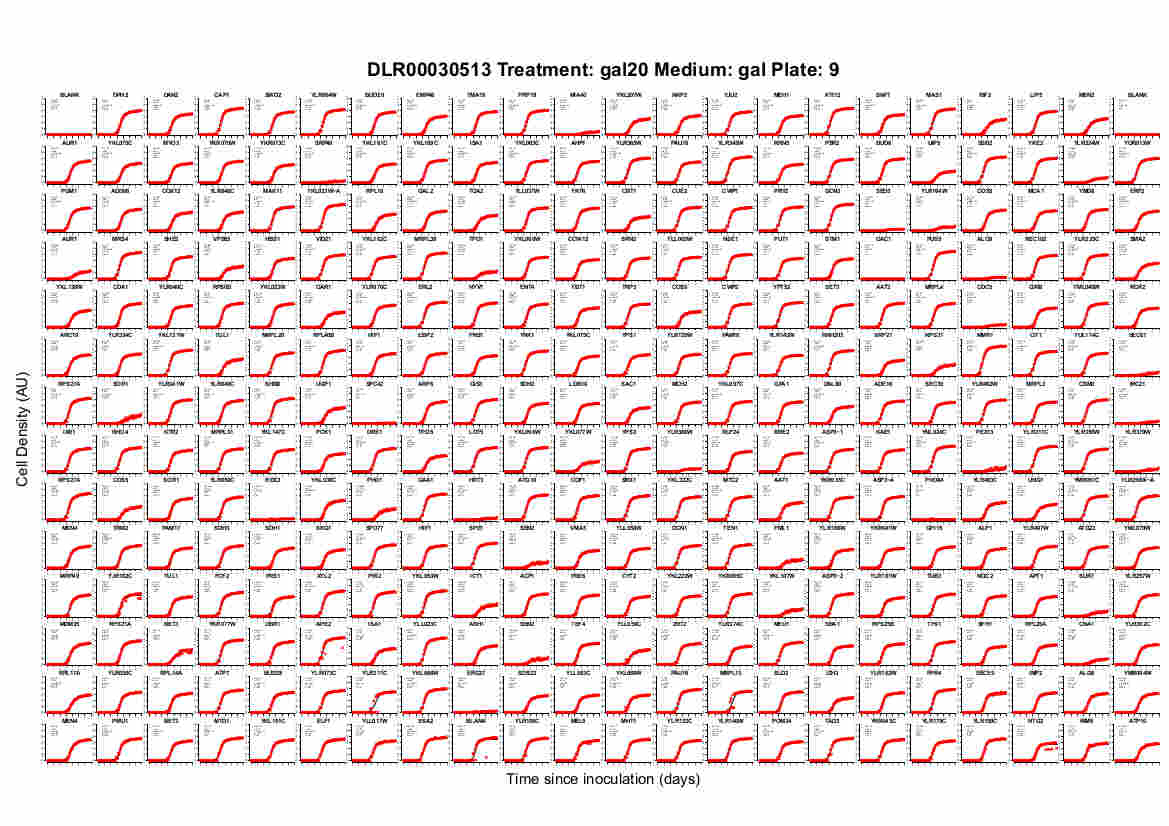
\includegraphics[width=\linewidth]{qfa_growth_array}
  \captionof{figure}{Growth curves, captured automatically by
    Colonyzer \citep{Lawless2010}, of 308 cultures in a QFA
    procedure. Reproduced ??with permission?? from \citet{Banks2012}.}
\end{Figure}
\begin{multicols}{2}

\end{multicols}
\graphicspath{{images_low_res/}}
\begin{Figure}
  \centering
  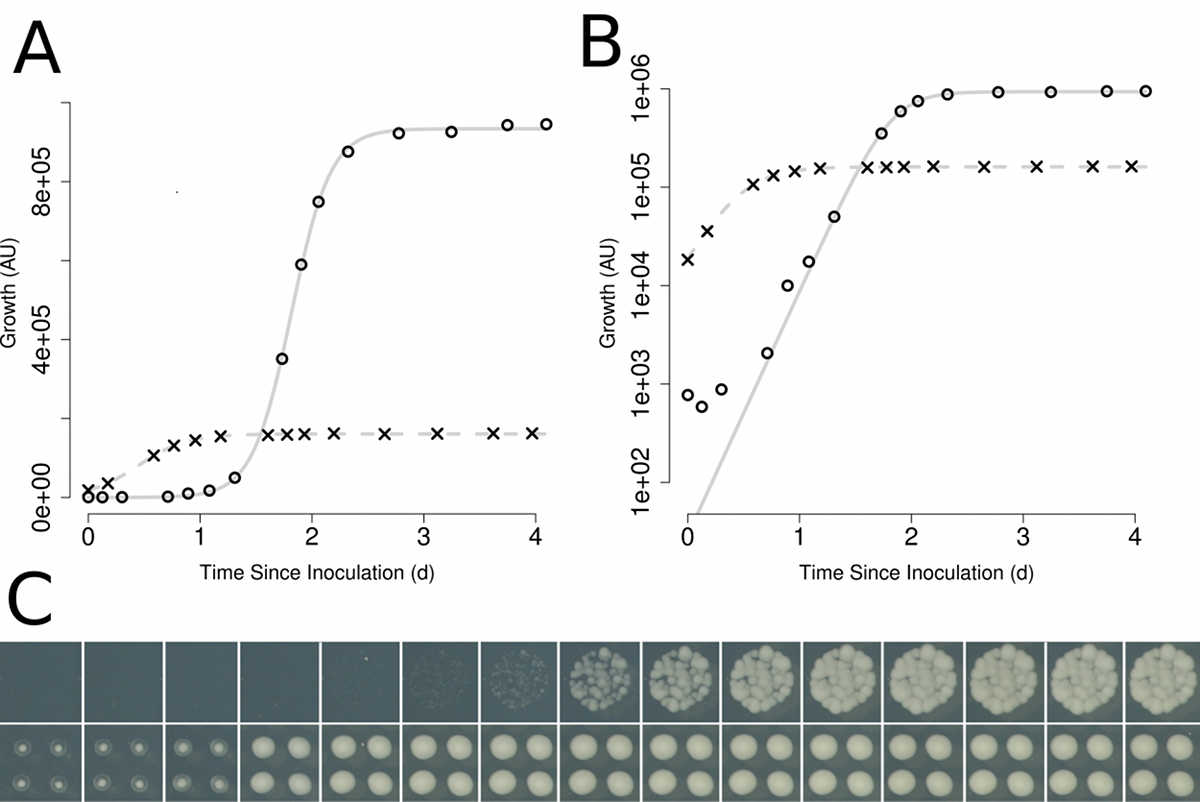
\includegraphics[width=\linewidth]{pin_v_spot_growth}
  \captionof{figure}{Fits of the logistic growth model, to cell
    density observations of yeast growing on solid agar, for spotted
    cultures (circles) and pinned cultures (crosses). In A) culture
    density is plotted on a linear scale. In B) culture density is
    plotted on a logarithmic scale. C) shows images of the spotted and
    pinned cultures corresponding to the data in A) \& B). Reproduced
    ??with permission?? from \citet{Lawless2010}.}
\end{Figure}
\begin{multicols}{2}
\subsection{Evidence of Competition and Signalling in QFA}

ethanol poisoning
quorum sensing


\subsection{Modelling Approaches}

\subsubsection{Mass Action Kinetics}
\subsubsection{The Logistic Growth Model}
\subsubsection{Fishers multiplicative model of genetic interactions}
\subsubsection{Hierarchical models and Bayesian inference}

\subsection{Inference of Genetic Interactions / Telomere Cap Defects}
\label{sec:genetic-interaction}
(Move to background section.
Motivated by the link between telomere shortening, ageing, and cancer
(refs?), \citet{Addinall2011} study the genetic interactions of
\textit{cdc13} which functions in telomere capping in the model
organism \textit{Saccharomyces cerevisiae}. If the power to predict
genetic interactions is improved in the reanalysis of data from
\citet{Addinall2011}, this may highlight new genes involved in these
processes and will also be relevant for investigations of other types
of genetic interaction and investigations using other types of
microbial organism.)


%%% Local Variables:
%%% mode: latex
%%% TeX-master: "proposal"
%%% End:
